\documentclass[11pt]{article}

% ===== 中文 XeLaTeX（Noto CJK，无需 ctex/xeCJK）=====
% 本机未安装 Noto CJK 时，自动改用 macOS 自带的宋体与冬青黑体
\usepackage{fontspec}
\IfFontExistsTF{Noto Serif CJK SC}{%
  \setmainfont{Noto Serif CJK SC}
  \setsansfont{Noto Sans CJK SC}
  \newfontfamily\cjkmono{Noto Sans Mono CJK SC}
}{%
  \setmainfont{Songti SC}
  \setsansfont{Hiragino Sans GB}[BoldFont={Hiragino Sans GB W6}]
  \newfontfamily\cjkmono{Hiragino Sans GB}
}
\XeTeXlinebreaklocale "zh"
\XeTeXlinebreakskip = 0pt plus 1pt

\usepackage[a4paper,margin=2.4cm]{geometry}
\usepackage{graphicx}
\usepackage{booktabs}
\usepackage{amsmath,amssymb}
\usepackage{array}
\usepackage{caption}
\usepackage{enumitem}
\usepackage{tikz}
\usetikzlibrary{arrows.meta,positioning,fit,backgrounds,calc}
\usepackage[hidelinks]{hyperref}
\usepackage{titlesec}
\usepackage{xcolor}

% 中文化标题名；中文无斜体，强调一律用黑体
\renewcommand{\abstractname}{\sffamily 摘要}
\renewcommand{\figurename}{图}
\renewcommand{\tablename}{表}
\renewcommand{\refname}{参考文献}
\let\emph\textbf

\captionsetup{font=small,labelfont=bf}
\setlist{nosep,leftmargin=1.6em}
\titleformat{\section}{\large\bfseries\sffamily}{\thesection}{0.6em}{}
\titleformat{\subsection}{\normalsize\bfseries\sffamily}{\thesubsection}{0.6em}{}

\newcommand{\unit}[1]{\,\mathrm{#1}}

% 配色
\definecolor{cq}{HTML}{4E79A7}
\definecolor{ce}{HTML}{59A14F}
\definecolor{cc}{HTML}{F28E2B}
\definecolor{cg}{HTML}{ECECEC}

\title{\sffamily\bfseries 量子随机数池：\\用含噪云端量子真机无损驱动大语言模型解码}
\author{基于逻辑比特云 QZ03 超导量子处理器与 stories15M 预训练模型}
\date{2026 年 11 月}

\begin{document}
\maketitle

\begin{abstract}
\noindent
在整条大语言模型（LLM）推理流水线中，随机数是\emph{唯一一个硬件噪声不构成错误}的环节——噪声只表现为比特偏置，
可由提取器完全消除。据此我们让一台含噪、未纠错的小型云端量子真机，第一次端到端驱动真实预训练 LLM 的解码：
QPU 离线产生随机比特、经 Toeplitz 提取入池，采样器逐 token 取用，GPU 前向不变、秒级 QPU 延迟不进入推理路径。
这同时关闭两道缺口：生产系统默认的伪随机数可由输出反推（我们实测观测 624 个输出即 100\% 逐字复现后续生成），
以及进入算力中心的量子算力在推理中无处落地。在逻辑比特云 QZ03（35 物理比特、无纠错）上驱动 stories15M：
原始真机比特 NIST SP 800-22 检验通过 2/11、提取后 \emph{11/11 全部通过}；采样的分布保真度与多样性和 MT19937、
CSPRNG 一致（token 频率相关 0.997--0.998），为\emph{无损替换}；物理来源使上述预测攻击退化为盲猜；单台设备支撑
约 \emph{1500 token/s} 的解码采样。据我们所知，这是通用云端门模型量子真机首次端到端驱动真实预训练 LLM 解码、
并完成随机性—安全—吞吐—成本全链路评测的公开案例。
\end{abstract}

\section{引言}
在整条 LLM 推理流水线中，随机数是\emph{唯一一个硬件噪声不构成错误}的环节。矩阵乘里噪声逐层累积、结果崩坏
（附录 A：单注意力头打分与精确值相关系数仅 0.52）；而随机数本就是量子测量的原生产物，噪声在此只表现为比特偏置，
只要估出最小熵，提取器就能把它\emph{完全消除}。据此我们让一台 35 物理比特、未纠错的云端量子真机，第一次端到端
驱动真实预训练 LLM 的解码：QPU 离线产生随机比特，经 Toeplitz 提取入池，采样器逐 token 取用；GPU 前向不变，
秒级 QPU 延迟不进入推理路径（\S\ref{sec:design}，图~\ref{fig:arch}）。

这一个切入点同时回答两道现实缺口。\textbf{其一，生成的核心是采样}：温度 $>0$ 时每个 token 都由一个随机数在分布
上反查决定，而在线 LLM 默认用伪随机数（MT19937 即 NumPy/PyTorch CPU 默认），其状态可由输出反推——
\S\ref{sec:attack} 我们实测观测 624 个输出即可 100\% 逐字复现后续生成，这是部署在生产里、从未在\emph{源头}关闭
的信任缺口。\textbf{其二，进入算力中心的量子算力在推理里无处落地}：把矩阵乘搬上量子线路，逐字复现每位置约需
$4.4\times10^{10}$ shots（附录 A）、容错编译每 token 约 $2\times10^{10}$ Toffoli，今天走不通。用物理测量产生
解码随机数恰落在两缺口交点——无种子、无可反推状态，从源头堵上其一；含噪小机即可胜任，落实其二。

现有把量子随机数接入 LLM 的工作，或依赖专用光子硬件~\cite{seedhijack}、或停留在玩具词表~\cite{tuna9}、
或未经系统评测~\cite{qrsampler}。据我们所知，这是\emph{通用云端门模型量子真机首次端到端驱动真实预训练 LLM}
（而非玩具、非模拟器、非专用光子）的解码。在逻辑比特云 QZ03 上驱动 stories15M，取得四项结果：
\begin{itemize}
  \item \emph{含噪比特变为合格随机源}（\S\ref{sec:rng}）：原始比特“为 1”的频率为 0.452、NIST 检验通过 2/11；
        经流水线提取后频率 0.501，\emph{11/11 全部通过}。
  \item \emph{无损即插即用}（\S\ref{sec:fidelity}）：分布保真度（卡方、KS、总变差）与生成多样性均与 MT19937、
        CSPRNG 一致，token 频率相关系数 0.997--0.998。
  \item \emph{从源头消除状态还原攻击面}（\S\ref{sec:attack}）：对推理栈默认的 MT19937，观测 624 个输出即可
        100\% 预测后续 token；量子随机数池无状态可窃、无种子可泄，攻击者降至盲猜基线。
  \item \emph{单台设备吞吐够用}（\S\ref{sec:cost}）：35 比特 QZ03 的纯执行产率为 $2.40\times10^4$ 可用 bit/s，
        可支撑约 1500 token/s 的解码采样。
\end{itemize}

\section{相关工作}
\textbf{量子随机数（QRNG）用于 LLM。} 与本文最接近的是 Seed Hijacking 一文~\cite{seedhijack}：它提出对 LLM 采样的
种子劫持攻击，并用\emph{专用光子} QRNG 卡（PCIe、预取数千万浮点数构成内存池）做防御，接入 GPT-2/Qwen2/DeepSeek，
实测该池化方案的中位延迟开销约 0.6\%。其硬件是专用光子器件而非通用量子处理器，且未报告生成质量的统计检验。
此外，有在云端门模型量子机 QuTech Tuna-9 上驱动 8 词词表玩具模型的演示~\cite{tuna9}，把 QRNG 作为采样插件的
工程尝试~\cite{qrsampler}，以及在 IBM 云超导设备上做 QRNG 的早期研究~\cite{ibmqrng}。

\textbf{可认证随机性。} JPMorganChase 与 Quantinuum 在 56 比特囚禁离子机 H2 上实现了基于随机电路采样的
可认证随机性，用超算验证，产出信息论意义上可证明的新鲜随机性~\cite{jpmc}。这类工作要求电路规模足以抵抗
经典模拟，硬件与验证代价极高。

\textbf{本文定位。} 我们把一台\emph{通用的、基于门模型的云端量子真机}用作随机数源，端到端驱动一个
\emph{真实预训练 LLM}（而非玩具词表）的解码，并给出随机性检验、与伪随机数的质量对照、安全攻防及吞吐/成本的
全链路真机实测。其中种子劫持攻击的思路取自~\cite{seedhijack}，本文在自己的门模型真机链路上复现并量化其后果。

\section{系统设计}
\label{sec:design}
整体架构把“产生随机数”与“消费随机数”解耦为三级流水线（图~\ref{fig:arch}）：

\begin{figure}[t]\centering
\begin{tikzpicture}[font=\sffamily\footnotesize,
  box/.style={draw,rounded corners=3pt,align=center,minimum height=1.05cm,inner sep=5pt},
  lbl/.style={font=\sffamily\scriptsize,text=black!55}]
\node[box,fill=cq!18,draw=cq] (q) {\textbf{量子侧}\\QZ03 离线补池\\$35$ qubit $\times$ Hadamard};
\node[box,fill=ce!18,draw=ce,right=0.9cm of q] (e) {\textbf{提取侧}\\最小熵定标\\Toeplitz 哈希};
\node[box,fill=black!4,draw=black!35,right=0.9cm of e] (p) {\textbf{随机数池}\\近均匀比特};
\node[box,fill=cc!18,draw=cc,right=0.9cm of p] (s) {\textbf{采样器}\\逆累积分布\\top-$p$};
\node[box,fill=black!4,draw=black!35,above=0.7cm of s] (g) {\textbf{GPU 前向}\\（不改动）};
\draw[-Stealth,thick] (q)--(e) node[midway,above,lbl]{原始 bit};
\draw[-Stealth,thick] (e)--(p) node[midway,above,lbl]{$u$};
\draw[-Stealth,thick] (p)--(s) node[midway,above,lbl]{$u$};
\draw[-Stealth,thick] (g)--(s) node[midway,right,lbl]{logits $P$};
\node[below=0.15cm of p,lbl,text width=8cm,align=center]{秒级 QPU 延迟被池吸收，不进入推理路径};
\draw[-Stealth,thick] (s.east)++(0.1,0) -- ++(0.7,0) node[right,font=\sffamily\scriptsize]{token};
\end{tikzpicture}
\caption{量子随机数池架构。量子侧与提取侧离线补池；采样器消费池中均匀数，与不改动的 GPU 前向并行；
QPU 延迟不在推理关键路径上。}
\label{fig:arch}
\end{figure}

\begin{enumerate}
  \item \textbf{量子侧（离线补池）}：在 QZ03 上重复执行“对 35 个物理比特各加一个 Hadamard 再测量”的电路，
        每条电路 1000 shots、产 $35\times1000$ 个原始比特。平台 SDK 在测量前插入读出校正门（\texttt{x21}），
        结果以 per-shot 位串（memory）返回。
  \item \textbf{提取侧（去偏）}：先做逐比特偏置与最小熵评估，再用 \textbf{Toeplitz 矩阵哈希}这一\emph{强随机性
        提取器}把带偏置、弱相关的原始比特压缩成接近理想均匀的输出（剩余哈希引理保证输出与均匀分布的统计距离
        $\le\varepsilon$，代价为损失 $2\log_2(1/\varepsilon)$ 比特）。
  \item \textbf{消费侧（解码）}：经典前向给出下一 token 的 logits，经温度与 top-$p$ 截断得到分布 $P$；从池中取
        一个均匀数 $u\in[0,1)$，用逆累积分布 $t=\min\{k:\sum_{i\le k}P_i>u\}$ 完成采样。每 token 消耗一个
        16-bit 均匀数。
\end{enumerate}

\section{实验}
平台：逻辑比特云 QZ03 超导量子处理器，35 个\textbf{物理比特}、网格拓扑、未做量子纠错（NISQ）；
CZ 两比特门保真度约 0.99--0.996，读出采用 measure2 方案。正因为是未纠错的物理比特，其原始读出才带有可观偏置
（\S\ref{sec:rng}），而这恰好落在提取器可消除的维度上。模型：stories15M（Karpathy 的 llama2.c 预训练模型，$1.52\times10^7$ 参数，
dim 288 / 6 层 / 6 头 / 词表 32000），\emph{不重新训练}。

\subsection{含噪比特经提取通过全部随机性检验}
\label{sec:rng}
数据集：QZ03 上 20 条任务（每条 35 比特 $\times$ 1000 shots），共 $2\times10^4$ 次测量、$7\times10^5$ 原始比特。

\textbf{待消除的偏置。} 原始比特存在读出偏置——总体“为 1”频率 0.452，最低单比特 $p_1=0.179$（图~\ref{fig:bias}a）；
这正是提取环节要消除的对象。按 $H_\infty=-\log_2\max(p_0,p_1)$ 估计逐比特最小熵，并对 $p_{\max}$ 取 99\%
置信上界得\emph{保守}下界（图~\ref{fig:bias}b），最小熵率保守为 \emph{0.855 bit/bit}，提取率即据此确定。

\textbf{Toeplitz 提取。} 取 $\varepsilon=2^{-100}$、输入块 7000 bit、留 5\% 工程余量，设输出 5496 bit/块，
提取率 \emph{0.785}；对 100 个块共提取 $5.496\times10^5$ 比特，“为 1”频率回到 \emph{0.5011}。

\textbf{随机性检验。} 在等长前缀（$5.49\times10^5$ bit）上对原始与提取后比特各跑 NIST SP 800-22~\cite{nist22}
的 11 项（表~\ref{tab:nist}、图~\ref{fig:nist}）：原始比特通过 2/11，\emph{提取后 11/11 全部通过}。
标准提取环节把真机读出偏置完整转化为合格随机源。

\begin{figure}[t]\centering
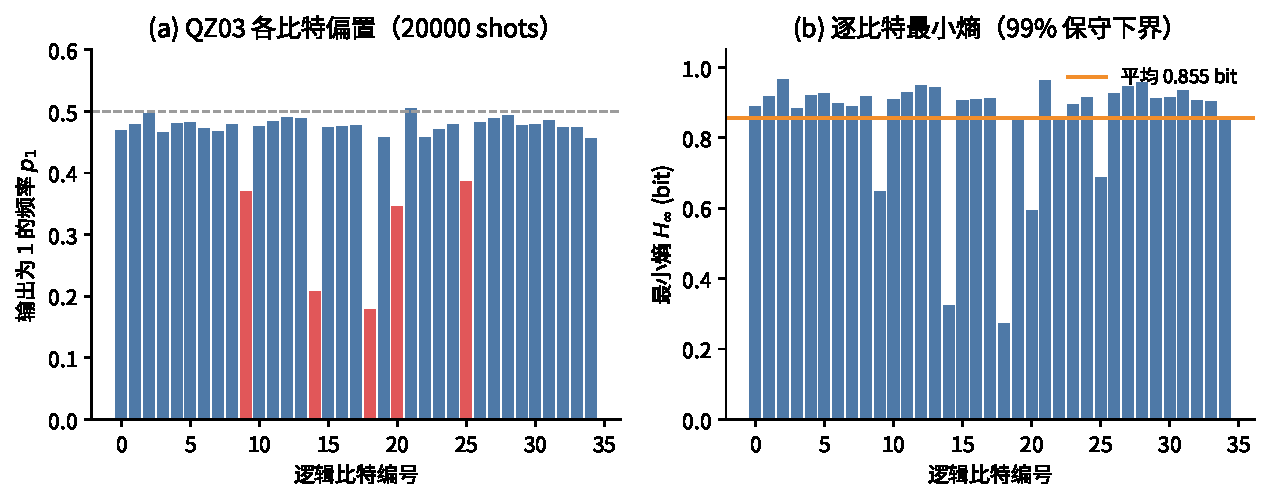
\includegraphics[width=\linewidth]{fig_bias.pdf}
\caption{提取前的原始偏置（a）与保守最小熵（b）：流水线据此确定 0.785 的提取率。
红色为偏离 0.5 超过 0.05 的比特。}
\label{fig:bias}
\end{figure}

\begin{figure}[t]\centering
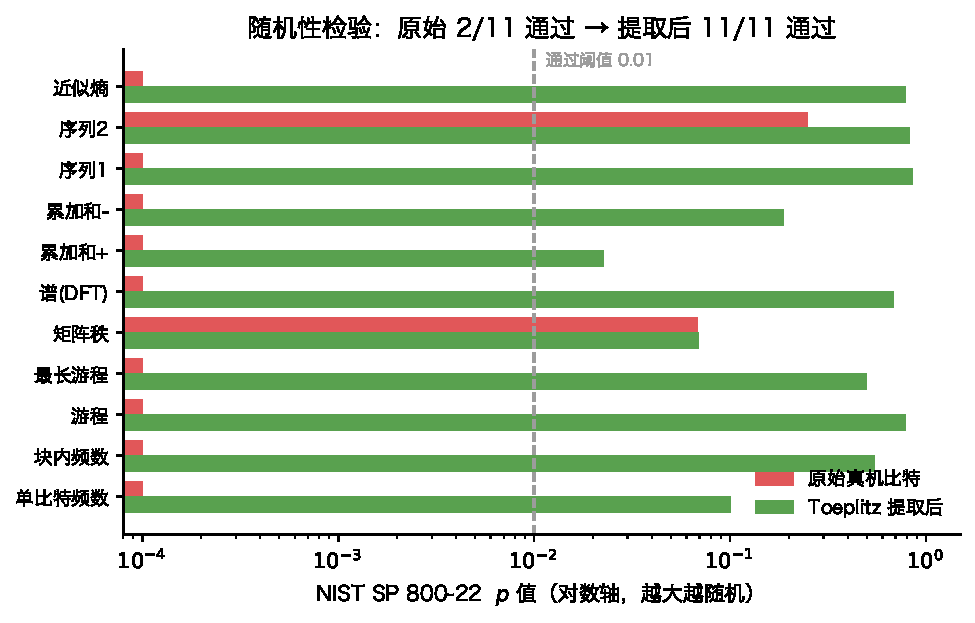
\includegraphics[width=0.86\linewidth]{fig_nist.pdf}
\caption{NIST SP 800-22 子集 $p$ 值（对数轴）。提取把 2/11 通过提升到 11/11 通过。}
\label{fig:nist}
\end{figure}

\begin{table}[t]\centering\small
\caption{NIST SP 800-22 子集 $p$ 值（$p\ge0.01$ 视为通过）。}
\label{tab:nist}
\begin{tabular}{lcc}
\toprule
检验项 & 原始真机比特 & Toeplitz 提取后 \\
\midrule
单比特频数 (Frequency) & 0.0000 & 0.1007 \\
块内频数 (Block Frequency) & 0.0000 & 0.5482 \\
游程 (Runs) & 0.0000 & 0.7900 \\
块内最长游程 (Longest Run) & 0.0000 & 0.4954 \\
二元矩阵秩 (Matrix Rank) & 0.0681 & 0.0694 \\
离散傅里叶谱 (DFT) & 0.0000 & 0.6864 \\
累加和-正向 (Cusum fwd) & 0.0000 & 0.0225 \\
累加和-反向 (Cusum bwd) & 0.0000 & 0.1884 \\
序列 (Serial) 1 & 0.0000 & 0.8584 \\
序列 (Serial) 2 & 0.2475 & 0.8287 \\
近似熵 (Approx. Entropy) & 0.0000 & 0.7864 \\
\midrule
\textbf{通过数} & \textbf{2/11} & \textbf{11/11} \\
\bottomrule
\end{tabular}
\end{table}

\subsection{无损即插即用：质量与伪随机数一致}
\label{sec:fidelity}
把三种随机源——量子随机数池（QRNG）、梅森旋转（MT19937，Python 标准库）、操作系统密码学随机数（CSPRNG，
\texttt{os.urandom}）——统一量化为 16-bit 均匀数，接入 stories15M 的 top-$p$ 采样（提示
“Once upon a time, there was a little”，温度 1.0，top-$p$ 0.9）。

\textbf{分布保真度。} 对首个新 token 的定分布 $P$，用三种源各抽 $1.5\times10^4$ 次。采样误差的参照系是\emph{理想
采样本身的噪声底}：同样次数的理想多项抽样，其与 $P$ 的总变差距离均值为 0.0043、95\% 区间 $[0.0013,0.0093]$。
三种源的总变差全部落在该区间内，量子池的 0.0044 正是理想采样的典型值（表~\ref{tab:fidelity}）。卡方与 KS 的
$p$ 值用于判断是否通过（均 $\gg0.01$），不用于源间排名。

\begin{table}[t]\centering\small
\caption{分布保真度（$N=1.5\times10^4$ 次抽样）。TV 的判据是理想采样噪声底，非源间比较。}
\label{tab:fidelity}
\begin{tabular}{lccc}
\toprule
随机源 & 卡方 $p$ & KS $p$ & 总变差 TV \\
\midrule
QRNG（QZ03 真机池） & 0.562 & 0.875 & 0.0044 \\
MT19937 & 0.944 & 0.113 & 0.0014 \\
CSPRNG & 0.361 & 0.505 & 0.0033 \\
\midrule
理想采样（参照） & --- & --- & 0.0043\;$[0.0013,0.0093]$ \\
\bottomrule
\end{tabular}
\end{table}

\textbf{生成多样性。} 量子随机数池保持了与 PRNG/CSPRNG 相同的生成多样性。三种源各生成 500 条长 20 的续写，
distinct-$n$ 与唯一续写占比一致，任意两源的 token 频率相关系数达 0.997--0.998（表~\ref{tab:diversity}）。

\begin{table}[t]\centering\small
\caption{生成多样性（每源 500 条、长 20 的续写）。}
\label{tab:diversity}
\begin{tabular}{lcccc}
\toprule
随机源 & distinct-1 & distinct-2 & distinct-3 & 唯一续写占比 \\
\midrule
QRNG（QZ03 真机池） & 0.060 & 0.166 & 0.259 & 0.844 \\
MT19937 & 0.058 & 0.162 & 0.249 & 0.828 \\
CSPRNG & 0.059 & 0.165 & 0.257 & 0.846 \\
\midrule
\multicolumn{5}{l}{\footnotesize token 频率相关：QRNG--MT19937 0.997；QRNG--CSPRNG 0.998；MT19937--CSPRNG 0.998} \\
\bottomrule
\end{tabular}
\end{table}

\textbf{小结：} 把采样随机源换成量子真机，分布保真度、多样性与 token 频率均与成熟 PRNG/CSPRNG 一致，
不付出任何质量代价。

\subsection{关闭采样信任缺口：实证}
\label{sec:attack}
本节给出\S1 缺口一的实证闭环：先把“默认采样可被预测”从隐患坐实为可执行的攻击，再证明量子随机数池从\emph{源头}
把它关闭。

\textbf{缺口是真实可利用的。} MT19937 是 Python 标准库与 PyTorch CPU 端的默认随机源、也是 NumPy 旧版接口的
默认算法，其内部状态是 624 个 32-bit 字；观测到 624 个连续输出后，逐个做 tempering 逆变换即可还原状态，预测
此后\emph{全部}输出。在 LLM 场景里，这意味着攻击者能预测、乃至操纵模型将采样出的 token。该攻击思路由
~\cite{seedhijack} 提出，我们在门模型真机链路上首次把它贯通到生成端并量化其后果。

实测（图~\ref{fig:attack}）：采样源为 MT19937 时，攻击者观测 624 个 32-bit 输出后，
\begin{itemize}
  \item 对随后 200 个随机数的预测命中率 \emph{100\%}（200/200）；
  \item 对随后 30 个\emph{生成 token} 的预测命中率 \emph{100\%}（30/30），逐字复现受害者的生成：
        “girl named Lily. She loved going to the park with her mom and dad…”。
\end{itemize}
\textbf{量子随机数池把它关闭。} 换成 QZ03 真机随机数池后，攻击者无法从历史比特还原任何状态，对随后 token 的
命中率为 73.3\%，与“仅知道分布、盲猜”的碰撞基线 $\mathbb{E}\sum_i P_i^2=70.4\%$ 无统计差异（二项检验
$p=0.84$）\footnote{碰撞基线由模型在该提示下的输出分布决定，与随机源无关。}。即攻击者\emph{退化到只能盲猜}，
缺口被关闭。

\begin{figure}[t]\centering
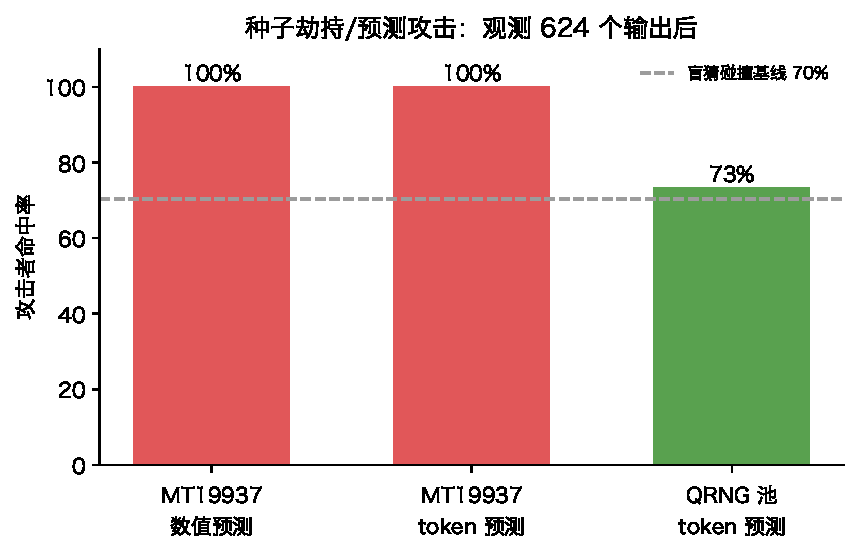
\includegraphics[width=0.62\linewidth]{fig_attack.pdf}
\caption{种子劫持/预测攻击。观测 624 个输出后 MT19937 被 100\% 预测；量子随机数池下攻击者命中率落在分布自身的
盲猜基线（虚线）。}
\label{fig:attack}
\end{figure}

\textbf{威胁模型与定位。} 物理随机源从\emph{源头}消除了这一类攻击面：它没有可还原的内部状态，也没有需要保密的
种子。密码学安全伪随机数生成器（CSPRNG）同样能抵抗状态还原，其安全性建立在种子保密与计算困难性假设之上；
量子随机数池的安全性则来自测量这一物理过程本身。二者对应不同的信任模型——量子源的特点是\emph{无状态可窃、
无种子可泄}。

\subsection{吞吐：单台设备支撑约 1500 token/s}
\label{sec:cost}
20 条任务的真机计量（平台返回的 \texttt{execution\_time} 与墙钟时间戳）给出表~\ref{tab:cost}。

\begin{table}[t]\centering\small
\caption{QZ03 随机数产出的吞吐、延迟与成本（20 条任务实测）。}
\label{tab:cost}
\begin{tabular}{ll}
\toprule
指标 & 数值 \\
\midrule
每条任务纯执行时间 & $1.15\pm0.24\unit{s}$（产 35000 原始 bit）\\
补池延迟（后台进行，不在推理路径上） & $1.4\unit{s}$（范围 $1$--$2\unit{s}$）\\
纯执行吞吐（原始 / 提取后） & $3.06\times10^4$ / $2.40\times10^4\unit{bit/s}$ \\
\textbf{可支撑的解码采样速率} & $\boldsymbol{\approx 1500}$ \textbf{token/s}（16 bit/token）\\
维持 1000 token/s 所需原始产率 & $2.04\times10^4\unit{bit/s}$（低于实测产率，留有余量）\\
总成本 / 单位成本 & ¥200（$5.50\times10^5$ 提取 bit）/ ¥364 每 Mbit \\
\bottomrule
\end{tabular}
\end{table}

\textbf{吞吐不构成瓶颈。} 单台 35 比特 QZ03 的纯执行产率已足以支撑约 1500 token/s 的解码采样，并对维持
1000 token/s 留有余量；池化设计把秒级 QPU 延迟与推理解耦，采样本身只是一次查表。\textbf{增量利用已部署的
量子算力。} 对已拥有量子算力的算力中心，本方案以每兆比特约 ¥364 的实测单价，让通用量子处理器在 LLM 推理
流程中承担确定的生产性负载，无需新增专用硬件，且对生成质量无损。

\section{适用范围与定位}
\label{sec:disc}
\begin{itemize}
  \item \textbf{随机性保证的来源。} 本文的随机性由 NIST SP 800-22 检验与 Toeplitz 提取器的剩余哈希引理保证。
        基于随机电路采样的可认证随机性~\cite{jpmc}要求电路规模足以抵抗经典模拟并配合第三方验证，35 比特 QZ03
        的电路可被经典模拟，因此本文不以可认证随机性为目标，二者是正交的两个方向。
  \item \textbf{提取器种子。} Toeplitz 矩阵由一段公开种子定义，本文由操作系统 CSPRNG 生成；对端到端量子来源
        有要求的部署，可改用独立可信随机源生成种子，流水线其余部分不变。
  \item \textbf{与模型规模无关的接口。} 随机数池只向采样器提供均匀数，与模型的参数量和结构无关，因此
        stories15M 足以验证从量子真机到生成 token 的完整链路。
\end{itemize}

\section{结论}
解码采样是 LLM 推理中天然对量子硬件噪声鲁棒的一环。基于这一观察，量子随机数池让一台 35 比特的含噪云端真机
端到端驱动预训练 LLM 的解码：含噪比特经提取通过全部 NIST 检验，生成质量无损，状态还原攻击面从源头消除，
单台设备的吞吐即可支撑约 1500 token/s。据我们所知，这是通用云端门模型量子真机首次端到端服务真实预训练 LLM
推理。在算力紧缺、同时拥有量子算力的现实设定下，\emph{量子随机数池}是把量子算力接入 LLM 推理最轻量、最鲁棒、
最直接的落点。

\appendix
\section{计算路径的代价}
\label{app:a}
本附录量化“把前向计算也搬上量子线路”的资源代价，支撑引言中“计算这条路今天走不通”的判断。我们把 stories15M 的
\emph{每一次矩阵-向量乘}（含注意力的 $q\cdot k$、$p\cdot V$）写成量子干涉线路：用形如
$\frac{1}{\sqrt{2R}}\sum_j|j\rangle(|0\rangle|\hat x\rangle+|1\rangle|\hat m_j\rangle)$ 的叠加态，
对辅助比特做 Hadamard 后测量，$P(j,0)-P(j,1)=\langle\hat x|\hat m_j\rangle/R$ 即给出内积（RMSNorm 增益与
RoPE 旋转并入权重）。在 Qiskit Aer 上：精确概率时 30/30 个 token 与经典逐字一致；每行 $10^6$ shots
（每位置 $4.4\times10^{10}$ shots）时仍 30/30 一致，$10^5$ 时第 25 个 token 起偏离——\emph{逐字复现的
shots 代价达 $10^{10}$ 量级}，这是计算路径不可行的根本原因。

在 QZ03 真机上实测第 0 层第 0 个注意力头的打分（48 维内积拆成 12 段 4 维 Hadamard 测试、10 段并行）：
单段 4 维余弦与理想值相关系数 0.90；合成 48 维打分相关系数 0.52、注意力分布总变差 0.55，而送回模型后下一个
词分布与精确值的总变差仅 0.017（单个低层头的误差被模型吸收）。即便单头误差可被吸收，逐字复现整条前向所需的
shots 规模仍远超解码随机数——两相对照，解码随机数池才是当下最直接可用的接入点。

\section*{复现}
配套代码与数据随本文提供：真机 QRNG 原始比特（\texttt{qz03\_qrng\_raw.json}，含 20 条任务 ID 与时间戳）、
随机性分析与提取（\texttt{analyze\_qrng.py}、\texttt{nist\_sts.py}）、采样对照（\texttt{qsample.py}）、
攻防演示（\texttt{attack.py}）、吞吐成本（\texttt{throughput.py}）、全前向量子化（\texttt{qfull.py}）。
真机平台：逻辑比特云（\texttt{cloud.logicalqubit.com}，SDK \texttt{lqcloud}）。

\begin{thebibliography}{9}
\bibitem{seedhijack} Seed Hijacking of LLM Sampling and Quantum Random Number Defense. arXiv:2605.08313 (2026).
\bibitem{tuna9} Quantum exordium for natural language processing: sampling on decoders, validated on QuTech Tuna-9 (T-9) hardware（8 词词表玩具演示）.
\bibitem{qrsampler} Quantum-random vLLM sampler (qr-sampler). \texttt{github.com/alchemystack/Quantum-random-vLLM-sampler}.
\bibitem{ibmqrng} K. Tamura, Y. Shikano. Quantum Random Numbers generated by the Cloud Superconducting Quantum Computer. arXiv:1906.04410 (2019).
\bibitem{jpmc} Certified randomness using a trapped-ion quantum processor (JPMorganChase \& Quantinuum H2, 56 qubits). Nature (2025).
\bibitem{nist22} A. Rukhin et al. A Statistical Test Suite for Random and Pseudorandom Number Generators. NIST SP 800-22 Rev.\,1a (2010).
\bibitem{nist90b} M. Turan et al. Recommendation for the Entropy Sources Used for Random Bit Generation. NIST SP 800-90B (2018).
\end{thebibliography}

\end{document}
